\section{CTCLSynchronize\-Command  Class Reference}
\label{classCTCLSynchronizeCommand}\index{CTCLSynchronizeCommand@{CTCLSynchronize\-Command}}
{\tt \#include $<$CTCLSynchronize\-Command.h$>$}

Inheritance diagram for CTCLSynchronize\-Command::\begin{figure}[H]
\begin{center}
\leavevmode
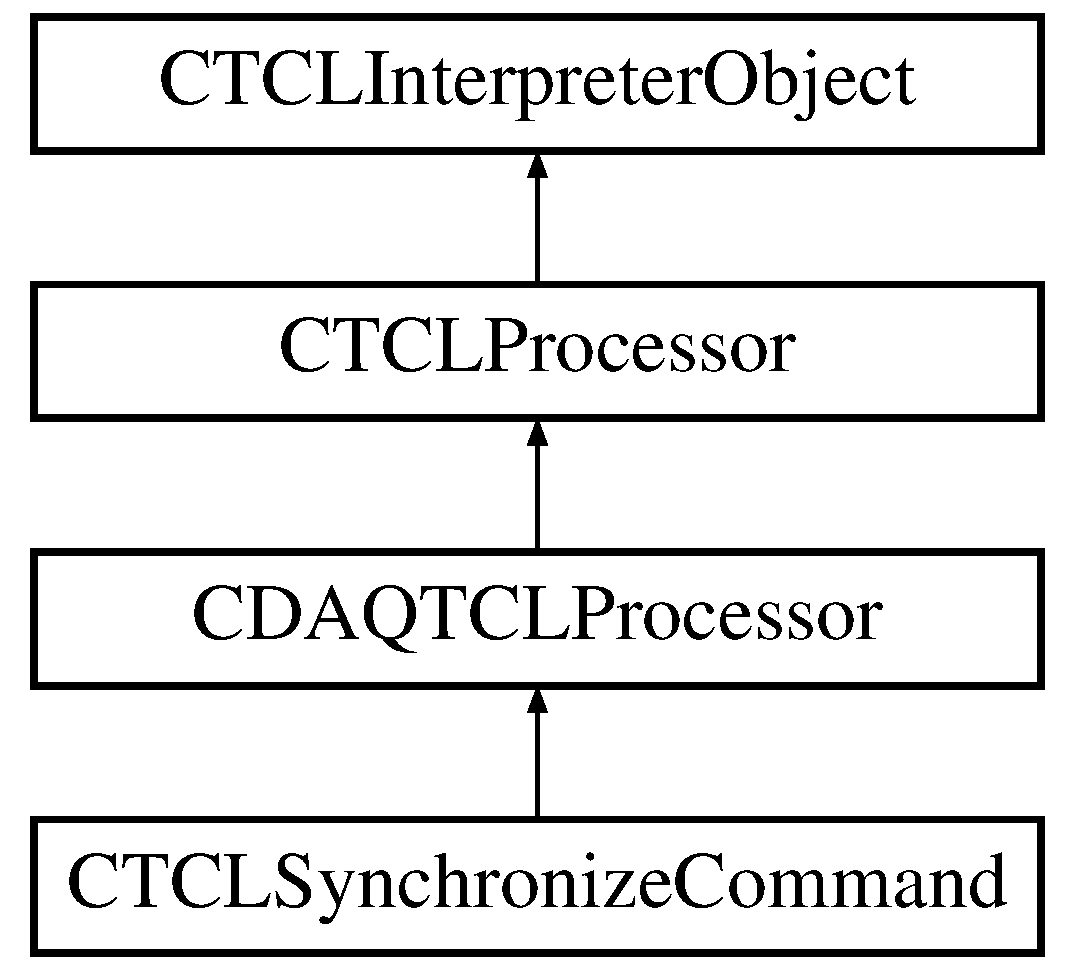
\includegraphics[height=4cm]{classCTCLSynchronizeCommand}
\end{center}
\end{figure}
\subsection*{Public Methods}
\begin{CompactItemize}
\item 
{\bf CTCLSynchronize\-Command} ({\bf CTCLInterpreter} $\ast$p\-Interp)
\item 
{\bf $\sim$CTCLSynchronize\-Command} ()
\begin{CompactList}\small\item\em Base class destructor does the work.\item\end{CompactList}\item 
int {\bf operator==} (const CTCLSynchronize\-Command \&a\-CTCLSynchronize\-Command) const
\begin{CompactList}\small\item\em Operator== Equality Operator.\item\end{CompactList}\item 
virtual int {\bf operator()} ({\bf CTCLInterpreter} \&r\-Interp, {\bf CTCLResult} \&r\-Result, int n\-Arguments, char $\ast$p\-Arguments[$\,$])
\end{CompactItemize}
\subsection*{Private Methods}
\begin{CompactItemize}
\item 
{\bf CTCLSynchronize\-Command} (const CTCLSynchronize\-Command \&a\-CTCLSynchronize\-Command)
\begin{CompactList}\small\item\em Copy Constructor private, and unimplemented.\item\end{CompactList}\item 
CTCLSynchronize\-Command \& {\bf operator=} (const CTCLSynchronize\-Command \&a\-CTCLSynchronize\-Command)
\begin{CompactList}\small\item\em Operator= Assignment Operator Private and unimplemented.\item\end{CompactList}\end{CompactItemize}


\subsection{Detailed Description}
Implements a Tcl command extension sync \{script\}

The script parameter is simply evaluated. Since this class is derived from {\bf CDAQTCLProcessor} {\rm (p.\,\pageref{classCDAQTCLProcessor})}, however the script is executed syncrhonized to the application's global mutex. Since the global mutex supports recursive locking, it is legal for the script to have synchronized commands embedded within its body. 



Definition at line 308 of file CTCLSynchronize\-Command.h.

\subsection{Constructor \& Destructor Documentation}
\index{CTCLSynchronizeCommand@{CTCLSynchronize\-Command}!CTCLSynchronizeCommand@{CTCLSynchronizeCommand}}
\index{CTCLSynchronizeCommand@{CTCLSynchronizeCommand}!CTCLSynchronizeCommand@{CTCLSynchronize\-Command}}
\subsubsection{\setlength{\rightskip}{0pt plus 5cm}CTCLSynchronize\-Command::CTCLSynchronize\-Command ({\bf CTCLInterpreter} $\ast$ {\em p\-Interp})\hspace{0.3cm}{\tt  [inline]}}\label{classCTCLSynchronizeCommand_a0}


Constructs the command. We only need an interpreter as the command name is fixed as \char`\"{}sync\char`\"{} 

Definition at line 314 of file CTCLSynchronize\-Command.h.\index{CTCLSynchronizeCommand@{CTCLSynchronize\-Command}!~CTCLSynchronizeCommand@{$\sim$CTCLSynchronizeCommand}}
\index{~CTCLSynchronizeCommand@{$\sim$CTCLSynchronizeCommand}!CTCLSynchronizeCommand@{CTCLSynchronize\-Command}}
\subsubsection{\setlength{\rightskip}{0pt plus 5cm}CTCLSynchronize\-Command::$\sim$CTCLSynchronize\-Command ()\hspace{0.3cm}{\tt  [inline]}}\label{classCTCLSynchronizeCommand_a1}


Base class destructor does the work.



Definition at line 318 of file CTCLSynchronize\-Command.h.\index{CTCLSynchronizeCommand@{CTCLSynchronize\-Command}!CTCLSynchronizeCommand@{CTCLSynchronizeCommand}}
\index{CTCLSynchronizeCommand@{CTCLSynchronizeCommand}!CTCLSynchronizeCommand@{CTCLSynchronize\-Command}}
\subsubsection{\setlength{\rightskip}{0pt plus 5cm}CTCLSynchronize\-Command::CTCLSynchronize\-Command (const CTCLSynchronize\-Command \& {\em a\-CTCLSynchronize\-Command})\hspace{0.3cm}{\tt  [private]}}\label{classCTCLSynchronizeCommand_c0}


Copy Constructor private, and unimplemented.



\subsection{Member Function Documentation}
\index{CTCLSynchronizeCommand@{CTCLSynchronize\-Command}!operator()@{operator()}}
\index{operator()@{operator()}!CTCLSynchronizeCommand@{CTCLSynchronize\-Command}}
\subsubsection{\setlength{\rightskip}{0pt plus 5cm}int CTCLSynchronize\-Command::operator() ({\bf CTCLInterpreter} \& {\em r\-Interp}, {\bf CTCLResult} \& {\em r\-Result}, int {\em n\-Arguments}, char $\ast$ {\em p\-Arguments}[$\,$])\hspace{0.3cm}{\tt  [virtual]}}\label{classCTCLSynchronizeCommand_a3}


Executes the script passed as argv[1] synchronized to the appliication's global mutex. Note that the Lack of an Argv[1] is not an error, no action will be performed, but the mutex will have been locked and unlocked.\begin{Desc}
\item[Parameters: ]\par
\begin{description}
\item[{\em 
r\-Interp}]is the interpreter on which the command is to execute. \item[{\em 
r\-Result}]is the result string to be filled in by the script. \item[{\em 
n\-Arguments}]is the number of command line arguments. \item[{\em 
p\-Arguments}]is a char$\ast$$\ast$ command parameter list. \end{description}
\end{Desc}


Implements {\bf CTCLProcessor} {\rm (p.\,\pageref{classCTCLProcessor_a7})}.

Definition at line 307 of file CTCLSynchronize\-Command.cpp.

References CTCLInterpreter::Eval().\index{CTCLSynchronizeCommand@{CTCLSynchronize\-Command}!operator=@{operator=}}
\index{operator=@{operator=}!CTCLSynchronizeCommand@{CTCLSynchronize\-Command}}
\subsubsection{\setlength{\rightskip}{0pt plus 5cm}CTCLSynchronize\-Command\& CTCLSynchronize\-Command::operator= (const CTCLSynchronize\-Command \& {\em a\-CTCLSynchronize\-Command})\hspace{0.3cm}{\tt  [private]}}\label{classCTCLSynchronizeCommand_c1}


Operator= Assignment Operator Private and unimplemented.

\index{CTCLSynchronizeCommand@{CTCLSynchronize\-Command}!operator==@{operator==}}
\index{operator==@{operator==}!CTCLSynchronizeCommand@{CTCLSynchronize\-Command}}
\subsubsection{\setlength{\rightskip}{0pt plus 5cm}int CTCLSynchronize\-Command::operator== (const CTCLSynchronize\-Command \& {\em a\-CTCLSynchronize\-Command}) const\hspace{0.3cm}{\tt  [inline]}}\label{classCTCLSynchronizeCommand_a2}


Operator== Equality Operator.



Definition at line 327 of file CTCLSynchronize\-Command.h.

References CTCLProcessor::operator==().

The documentation for this class was generated from the following files:\begin{CompactItemize}
\item 
{\bf CTCLSynchronize\-Command.h}\item 
{\bf CTCLSynchronize\-Command.cpp}\end{CompactItemize}
